% !TeX spellcheck = cs_CZ
%{\tikzset{external/prefix={tikz/FYZII/}}
% \tikzset{external/figure name/.add={ch06_}{}}
%---------------------------------------------------------------------------------------------------
% file fey1ch08.tex
%---------------------------------------------------------------------------------------------------
%====================Kapitola: Elektrostatická energie =============================================
\setchaptertoc
\chapter{Elektrostatická energie}\label{fyz:IIchapVI}
  \section{Elektrostatická energie nábojů. Homogenní koule}\label{fyz:IIchapVIsecI}
    Jedním z nejzajímavějších a nejužitečnějších objevů v mechanice byl zákon zachování energie.
    Vzorce pro kinetickou a potenciální energii mechanické soustavy nám pomáhají objevit souvislosti
    mezi stavy soustavy ve dvou různých časech, aniž bychom museli vnikat do podrobností toho, co se
    mezi tím děje. Nyní se chceme zabývat energií elektrostatických soustav. I v nauce o elektřině
    bude princip zachování energie užitečný při objevování mnoha zajímavých věcí.

    Zákon o energii vzájemného působení je v elektrostatice velmi jednoduchý; vlastně jsme ho již
    probírali. Představte si, že máme dva náboje \(q_1\) a \(q_2\) vzdálené od sebe o \(r_{12}\).
    Tato soustava se vyznačuje nějakou energií, neboť na to, aby se oba náboje přivedly do jejich
    současné vzájemné polohy, bylo třeba vynaložit určité množství práce. Práci, která je vykonána
    při přiblížení dvou nábojů z velké vzdálenosti, jsme už počítali. Je rovna
    \begin{equation}\label{fyz:eq868}
      \dfrac{q_1q_2}{4πϵ_0r_{12}}.      
    \end{equation}
    Kromě toho z principu superpozice víme, že v případě mnoha nábojů je celková síla působící na
    každý z nich rovna součtu sil, kterými na něj působí všechny ostatní náboje. Z toho vyplývá, že
    celková energie soustavy více nábojů je rovna součtu členů pocházejících ze vzájemné interakce
    každého páru nábojů. Jsou-li \(q_i\) a \(q_j\) některé dva z těchto nábojů a \(r_{12}\) je
    vzdálenost mezi nimi (\ref{fyz:fig178}), energie tohoto páruje
    \begin{equation}\label{fyz:eq869}
      \dfrac{q_iq_j}{4πϵ_0r_{ij}}.      
    \end{equation}

    \begin{figure}[ht!]  %\ref{fyz:fig178}
      \centering
      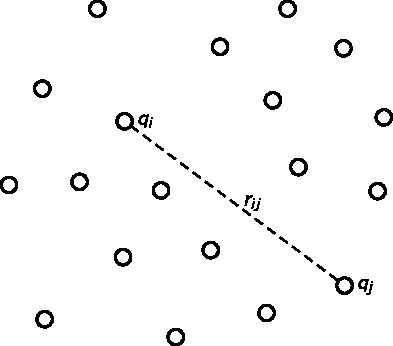
\includegraphics[width=0.6\linewidth]{fyz_fig178.pdf}
      \caption{Elektrostatická energie soustavy částic je rovna součtu elektrostatických energií
              všech párů částic v soustavě (\cite[s.~140]{Feynman02}).}
      \label{fyz:fig178}
    \end{figure}

    Výsledná elektrostatická energie \(W\) je součtem energií všech možných párů nábojů v soustavě:
    \begin{equation}\label{fyz:eq870}
      W=\sum_{\mathclap{\substack{\text{všechny}\\\text{páry}}}}\dfrac{q_iq_j4πϵ_0}{r_{ij}}.
    \end{equation}
    Jde-li o rozdělení nábojů specifikované hustotou náboje \(ρ\), je samozřejmě nutné nahradit sumu
    ve vzorci (\ref{fyz:eq870}) integrálem.

    My se budeme touto energií zabývat ze dvou hledisek. Jedním je \emph{využití} pojmu energie v
    elektrostatických úlohách a druhým jsou různé způsoby výpočtu energie. Někdy je snazší vypočítat
    práci vykonanou v nějakém speciálním případě, než vyčíslit sumu nebo příslušný integrál ve
    vzorci (\ref{fyz:eq870}). Jako příklad vypočtěme energii potřebnou na shromáždění náboje do
    koule s homogenní hustotou náboje. Je rovna práci vykonané při přibližování nábojů z nekonečna.

    Představte si, že kouli vytváříme postupným přikládáním tenkých kulových slupek s
    infinitezimální tloušťkou na sebe. V každém stádiu tohoto procesu bereme malé množství náboje a
    přikládáme jej ve tvaru tenké kulové slupky sahající od \(r\) do \(r + \dd{r}\).

    \begin{figure}[ht!]  %\ref{fyz:fig179}
      \centering
      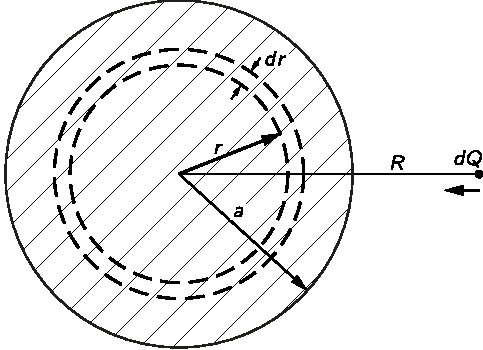
\includegraphics[width=0.6\linewidth]{fyz_fig179.pdf}
      \caption{Energii homogenně nabité koule můžeme počítat tak, že si představíme kouli, jako by
              byla složena ze vzájemně na sebe přiléhajících kulových slupek.
              (\cite[s.~141]{Feynman02}).}
      \label{fyz:fig179}
    \end{figure}

    Pokračujeme tak dlouho, dokud nedosáhneme konečného poloměru a (obr. \ref{fyz:fig179}). Je-li
    náboj koule ve stádiu, kdy byla vytvořena do poloměru \(r\), je při přinášení dalšího náboje
    \(\dd{Q}\) vykonávána práce.
    \begin{equation}\label{fyz:eq871}
      \dd{W}=\dfrac{Q}{r^4πϵ_0r}\dd{Q}.
    \end{equation}
    Je-li hustota náboje v kouli \(ρ\), náboj \(Q_r\) je
    \begin{equation*}
      Q_r=ρ\cdot\dfrac{4}{3}πr^3,
    \end{equation*}
    a náboj \(\dd{Q}\) je vyjádřen takto:
    \begin{equation*}
      \dd{Q}=ρ⋅4πr^2\dd{r}.
    \end{equation*}
    Rovnost (\ref{fyz:eq871}) pak získá tvar
    \begin{equation}\label{fyz:eq872}
      \dd{W}=\dfrac{4πρ^2r^4\dd{r}}{3ϵ_0}.
    \end{equation}
    Celková energie potřebná na vytvoření koule je rovna integrálu \(\dd{W}\) od \(r = 0\) do \(r =
    a\), tj.
    \begin{equation}\label{fyz:eq873}
      W=\dfrac{4πρ^2a^5}{15ϵ_0}.
    \end{equation}
    Chceme-li výsledek vyjádřit pomocí celkového náboje \(Q\) koule, dostaneme
    \begin{equation}\label{fyz:eq874}
      W=\dfrac{3}{5}\dfrac{Q^2}{4πϵ_0a}.
    \end{equation}
    Energie je tedy přímo úměrná druhé mocnině celkového náboje a nepřímo úměrná poloměru. Vztah
    (\ref{fyz:eq874}) můžeme interpretovat také tak, že podle něj je střední hodnota veličiny
    (\(1/r_{ij}\)) pro všechny páry bodů v kouli \(3/5 a\).

  \twocolumn[\section{Energie kondenzátoru. Síly působící na nabité vodiče}\label{fyz:IIchapVIsecII}]
    Nyní uvažujme o energii potřebné k nabití kondenzátoru. Vezmeme-li od jednoho z vodičů tvořících
    kondenzátor náboj \(Q\) a přeneseme-li ho na druhý vodič, vznikne mezi nimi rozdíl potenciálů
    \begin{equation}\label{fyz:eq875}
      U = \dfrac{Q}{C},
    \end{equation}
    kde \(C\) je kapacita kondenzátoru. Kolik práce je vykonáno při nabíjení kondenzátoru? Budeme
    postupovat stejně jako v případě koule a představíme si, že kondenzátor se nabíjel přenášením
    náboje po malých částech \(\dd{Q}\), z jedné jeho desky na druhou. Na přenesení náboje
    \(\dd{Q}\) je spotřebována práce
    \begin{equation*}
      \dd{W} = U\dd{Q}.
    \end{equation*}
    Dosazením \(U\) z (\ref{fyz:eq875}) tento vztah získá tvar
    \begin{equation*}
      \dd{U} = \dfrac{Q\dd{Q}}{C}.
    \end{equation*}
    Když potom integrujeme od nulového do konečného náboje \(Q\) dostaneme
    \begin{align}
      W &= \dfrac{1}{2}\dfrac{Q^2}{C}.  \label{fyz:eq876}     \\
      \shortintertext{Tuto energii je možné napsat i ve tvaru}
      W &= \dfrac{1}{2}CU^2.            \label{fyz:eq877}
    \end{align} 

    Vzpomeneme-li si, že kapacita vodivé koule (vzhledem k nekonečnu) je
    \begin{equation*}
      C_{\text{koule}} = 4πϵ0a,
    \end{equation*}
    můžeme ze vzorce (\ref{fyz:eq876}) ihned dostat vztah pro energii nabité koule:
    \begin{equation}\label{fyz:eq878}
      W=\dfrac{1}{2}\dfrac{Q^2}{4πϵ_0a}.
    \end{equation}
    Ovšem toto je i vztah pro energii \emph{tenké kulové slupky} s celkovým nábojem \(Q\) tato
    energie představuje \(5/6\) energie homogenně nabité koule, vyjádřené vztahem (\ref{fyz:eq874}).

    Nyní se zabývejme aplikacemi pojmu elektrostatické energie. Zkoumejme následující otázky: Jaká
    síla působí mezi elektrodami kondenzátoru? Nebo: Jaký moment síly vzhledem k nějaké ose působí
    na nabitý vodič v přítomnosti jiného vodiče s opačným nábojem? Takové otázky lze snadno
    zodpovědět použitím našeho výsledku (\ref{fyz:eq877}) pro elektrostatickou energii kondenzátoru
    spolu s principem virtuální práce (viz kapitoly \ref{fyz:IchapII}, a \ref{fyz:chap_fey_work},
    díl \ref{part:FYZI}).

    Použijeme tuto metodu na určení síly působící mezi deskami rovinného kondenzátoru.
    Představíme-li si, že mezera mezi deskami se zvětšila o malou hodnotu \(\Delta z\), mechanická
    práce vynaložená vnější silou na posunutí desek byla
    \begin{equation}\label{fyz:eq879}
      ΔA=FΔz,
    \end{equation}
    kde \(F\) je síla působící mezi deskami. Tato práce musí být rovna změně elektrostatické energie
    kondenzátoru.

    Podle vztahu (\ref{fyz:eq876}) měl kondenzátor původně energii
    \begin{equation*}
      W = \dfrac{1}{2}\dfrac{Q^2}{C}.
    \end{equation*}
    Změna energie (nedopustíme-li, aby se náboj změnil) je
    \begin{equation}\label{fyz:eq880}
      ΔW=\dfrac{1}{2}Q^2Δ\left(\dfrac{1}{C}\right).
    \end{equation}
    Porovnáním (\ref{fyz:eq879}) a ({fyz:eq880}) dostaneme
    \begin{align}
      FΔz &=\dfrac{Q^2}{2}Δ\left(\dfrac{1}{C}\right). \label{fyz:eq881} \\
      \shortintertext{což je možné napsat ve tvaru}
      FΔz &=−\dfrac{Q^2}{2C^2}ΔC.                     \label{fyz:eq882}
    \end{align}
    Působící síla, samozřejmě, vyplývá z rozdělení nábojů na deskách, ale jak je vidět, nemusíme se
    starat o jejich detailní rozdělení; všechno, co potřebujeme, je obsaženo v kapacitě \(C\)

    \begin{figure}[ht!]  %\ref{fyz:fig180}
      \centering
      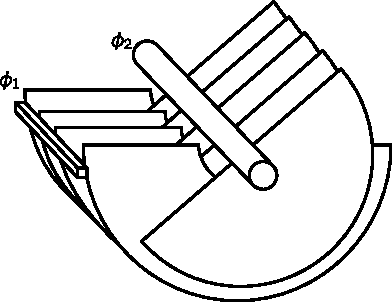
\includegraphics[width=0.6\linewidth]{fyz_fig180.pdf}
      \caption{Jaký moment síly působí na otočný kondenzátor? (\cite[s.~144]{Feynman02}).}
      \label{fyz:fig180}
    \end{figure}

    Je zřejmé, že tuto myšlenku lze rozšířit na vodiče jakéhokoliv tvaru a na ostatní složky síly.
    Ve vztahu (\ref{fyz:eq881}) zaměníme \(F\) složkou, kterou hledáme, a \(\Delta z\) nahradíme
    malým posunutím v odpovídajícím směru. Nebo máme-li elektrodu vyznačující se nějakou osou a je
    třeba najít moment síly \(τ\), napíšeme virtuální práci ve tvaru
    \begin{equation*}
      ΔA=τΔθ,
    \end{equation*}
    kde \(Δθ\) je malé \emph{úhlové posunutí}. V tomto případě musí \(Δ(1/C)\) přirozeně
    představovat změnu veličiny \(1/C\) příslušnou pootočení \(Δθ\). Tak bychom mohli najít moment
    působící na pohyblivé desky v otočném kondenzátoru takového typu, jako je na obr.
    \ref{fyz:fig181}.
    
    Vrátíme se ke speciálnímu případu kondenzátoru s rovnoběžnými rovinnými elektrodami. Pro jeho
    kapacitu můžeme použít vzorec odvozený v kapitole \ref{fyz:IIchapV}:
    \begin{equation}\label{fyz:eq883}
      \dfrac{1}{C}=\dfrac{d}{ϵ_0S},
    \end{equation}
    kde \(S\) je plošný obsah každé desky. Zvětšíme-li mezeru mezi deskami o \(\Delta z\), bude
    platit
    \begin{equation*}
      Δ\left(1C\right)=\dfrac{Δz}{ϵ_0S}.
    \end{equation*}
    Z rovnice (\ref{fyz:eq881}) dostaneme, že síla mezi deskami je
    \begin{equation}\label{fyz:eq884}
      F=\dfrac{Q^2}{2ϵ_0S}.
    \end{equation}
    Všimněme si výrazu (\ref{fyz:eq881}) trochu blíže a podívejme se, zda lze říci, jak tato síla
    vzniká. Vyjádříme-li náboj na jedná desce ve tvaru
    \begin{equation*}
      Q=σS,
    \end{equation*}
    vztah (\ref{fyz:eq884}) lze přepsat takto:
    \begin{equation*}
      F=\dfrac{1}{2}Q\dfrac{σ}{ϵ_0}.
    \end{equation*}
    Protože intenzita elektrického pole mezi deskami je
    \begin{equation*}
      E_0=\dfrac{σ}{ϵ_0},
    \end{equation*}
    máme
    \begin{equation}\label{fyz:eq885}
      F=\dfrac{1}{2}QE_0.
    \end{equation}

    Ihned bylo možné se dovtípit, že síla působící na jednu desku je rovna součinu náboje \(Q\) na
    desce a intenzity pole působícího na náboj. Dostali jsme však překvapující součinitel \(1/2\).
    Příčina spočívá v tom, že \(E_0\) není ta intenzita pole, která je v místě, kde jsou náboje.
    Když si představíme, že náboj zabírá tenkou vrstvu na povrchu desky, jak to znázorňuje obr.
    \ref{fyz:fig181}, intenzita pole se bude měnit od nuly na vnitřním okraji vrstvy do \(E_0\) v
    prostoru mimo desku.
    
    \begin{figure}[ht!]  %\ref{fyz:fig181}
      \centering
      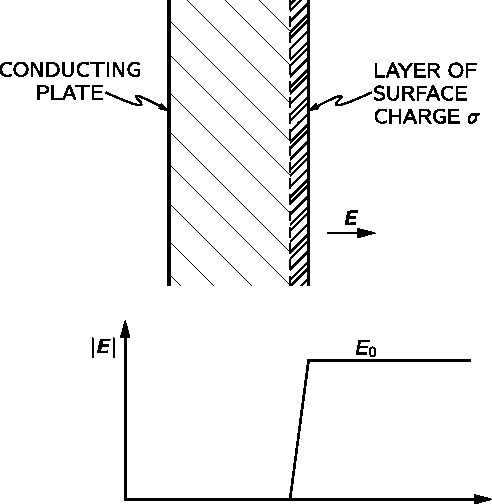
\includegraphics[width=0.8\linewidth]{fyz_fig181.pdf}
      \caption{Intenzita elektrického pole se změní při průchodu vrstvou plošného náboje
              existujícího na povrchu vodiče z nuly na hodnotu \(E_0 =
              \frac{\sigma}{\varepsilon_0}\) (\cite[s.~145]{Feynman02}).}
      \label{fyz:fig181}
    \end{figure}

    Střední intenzita působící na náboje je \(E_0/2\). To je důvod, proč ve vztahu (\ref{fyz:eq885})
    vystupuje součinitel \(1/2\).

    Je nutné, abychom si všimli, že při výpočtu virtuální práce jsme předpokládali, že náboj na
    kondenzátoru je stálý, tj. že kondenzátor není elektricky připojen k jiným tělesům, a tak se
    celkový náboj nemůže měnit. 
    
    Předpokládejme, že po dobu virtuálního přemístění by se kondenzátor udržoval na stálém rozdílu
    potenciálů. V tom případě bychom měli použít vztah
    \begin{equation*}
      W = \dfrac{1}{2}CU^2.
    \end{equation*}
    a místo (\ref{fyz:eq882}) bychom dostali
    \begin{equation*}
      FΔz=\dfrac{1}{2}U^2ΔC,
    \end{equation*}
    z čehož vyplývá stejně velká síla jako ze vztahu (\ref{fyz:eq882}) (neboť \(U= Q/C\)), ale s
    opačným znaménkem. Tím, že jsme kondenzátor odpojili od nabíjecího zdroje, síla mezi jeho
    elektrodami zajisté nezmění znaménko. Kromě toho víme, že dvě elektrody s opačnými elektrickými
    náboji se musí přitahovat. V druhém případě však byl princip virtuální práce použit nekorektně -
    nevzali jsme v úvahu virtuální práci vykonanou nabíjecím zdrojem. Aby se totiž při změně
    kapacity udržel stejný potenciál \(U\), je nutné, aby zdroj dodal náboj \(U\Delta C\). Tento
    náboj je však dodáván při potenciálu \(U\), takže práce konaná elektrickým systémem udržujícím
    neměnný potenciál, je \(U^2\Delta C\). Mechanická práce \(F\Delta z\) \emph{plus} elektrická
    práce \(U^2\Delta C\) spolu dávají změnu celkové energie kondenzátoru rovnou —
    \(\frac{1}{}U^2\Delta C\). Proto \(FΔz=−\frac{1}{2}V^2ΔC\) stejně jako předtím.
    
  \twocolumn[\section{Elektrostatická energie iontového krystalu}\label{fyz:IIchapVIsecIII}] 
  
    Nyní se zabývejme využitím pojmu elektrostatické energie v atomové fyzice. Síly mezi atomy nelze
    méřit snadno, ale často nás zajímají rozdíly energie mezi dvěma konfiguracemi atomů, např.
    energie chemických změn. Protože atomové síly jsou v podstatě elektrickými silami, chemické
    energie jsou z velké části právě elektrostatickými energiemi.
    
    Uvažujme například elektrostatickou energii iontové mřížky. Iontový krystal, tj. takový jako je
    krystal \ce{NaCl}, se skládá z kladných a záporných iontů, které je možné považovat za tuhé
    koule. Elektricky se přitahují, dokud se nezačnou vzájemně dotýkat; potom se uplatní odpudivá
    síla, která velmi prudce vzroste, pokusíme-li s eje přiblížit těsněji.
    
    Proto jako naše první přiblížení vezměme soustavu tuhých koulí, představující atomy v krystalu
    kuchyňské soli. Struktura krystalové mřížky byla určena pomocí ohybu rentgenového záření. Jde o
    kubickou mřížku (jako trojrozměrná šachovnice). Obr. \ref{fyz:fig182} ukazuje její řez.
    Vzdálenost mezi sousedními ion tyje \SI{0.281}{\nm} (=\SI{2.81e-10}{\m}).
    
    \begin{figure}[ht!]  %\ref{fyz:fig182}
      \centering
      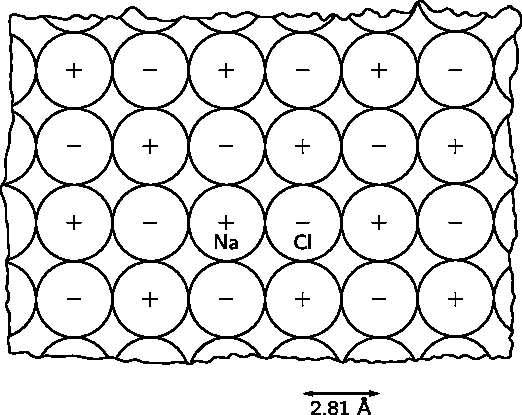
\includegraphics[width=0.6\linewidth]{fyz_fig182.pdf}
      \caption{Řez krystalem kuchyňské soli v atomovém měřítku. Šachovnicové uspořádání iontů \ce{Na} 
              a \ce{Cl} je stené v obou na sebe kolmých řezech krystalem (obr. \ref{fyz:fig013} díl
              \ref{part:FYZI}) (\cite[s.~146]{Feynman02}).}
      \label{fyz:fig182}
    \end{figure}

    Je-li náš obraz této soustavy správný, měli bychom být schopni provéřit jej tím, že si položíme
    následující otázku: Kolik energie je třeba, aby se všechny tyto ionty od sebe navzájem oddělily,
    tj. aby se krystal úplně rozbil na jednotlivé ionty? Tato energie bude rovna skupenskému teplu
    vypařování \ce{NaCl} zvětšená o energii potřebnou na disociaci molekul na ionty. Celková energie
    potřebná na rozdrobení \ce{NaCl} na ionty byla experimentálně určena jako \num{7.92}
    elektronvoltů na jednu molekulu. Použijeme-li převod
    \begin{equation*}
      \SI{1}{\electronvolt} = \SI{1.602e-19}{\joule}
    \end{equation*}
    a Avogadrovu konstantu jako počet molekul v jednom molu, tedy
    \begin{align*}
      N_0 &= \SI{6.02e23}{\per\mole},  \\
      \shortintertext{energii vypařování napíšeme takto:}
      W   &= \SI{7.64}{\joule\per\mole}.
    \end{align*}

    Je možné dostat tuto chemickou energii teoreticky vypočítáním množství práce potřebné k
    roztržení krystalu? Podle naší teorie představuje tato práce součet potenciálních energií všech
    iontových párů. Nejsnadnější cestou pro výpočet tohoto součtu je vybrat vždy konkrétní ion a
    počítat jeho potenciální energii vzhledem ke každému z ostatních iontů. Dostaneme tak
    \emph{dvojnásobek} energie připadající najeden ion, protože počítané energie budou náležet párům
    iontů. Potřebujeme-li, aby se vypočítaná energie vztahovala k jedinému konkrétnímu iontu, musíme
    vzít poloviční hodnotu. Ale ve skutečnosti potřebujeme energii připadající na \emph{jednu
    molekulu}, která obsahuje dva ionty, takže vypočtený součet bude přímo udávat energii
    připadající na molekulu.

    Energie iontu vzhledem k jednomu z jeho nebližších sousedů je rovna \(e^2/a\), kde
    \(e^2=q^2e/4πϵ_0\) a \(a\) je vzdálenost mezi středy obou iontů. (Uvažujeme jednovazné ionty.)
    Tato energie je rovna \SI{5.12}{\electronvolt}, což, jak už vidíme, by nám mělo poskytnout
    výsledek o řádově správné velikosti. Ale do nekonečné sumy, kterou potřebujeme spočítat, je
    ještě dlouhá cesta.

    Začněme sčítáním všech členů, které pocházejí od iontů ležících v jedné přímce.
    Předpokládáme-li, že ion označený \ce{Na} na obr. \ref{fyz:fig182} je naším konkrétním iontem,
    uvažme nejdříve ty ionty, které s ním leží na jedné vodorovné přímce. Nejbližší jsou dva záporně
    nabité ionty \ce{Cl}, každý ve vzdálenosti \(a\). Potom jsou dva kladné ionty ve vzdálenosti
    \(2a\) atd. Označíme-li energii, kterou dá tento součet \(W_1\), bude platit
    \begin{align*}
      W &= \dfrac{e^2}{a}\left(−\dfrac{2}{1}+\dfrac{2}{2}−\dfrac{2}{3}+\dfrac{2}{4}∓\cdots\right) \\
        &= −\dfrac{2e^2}{a}\left(1−\dfrac{1}{2}+\dfrac{1}{3}−\dfrac{1}{4}±\cdots\right).
    \end{align*}
    Tato řada konverguje pomalu, takže je těžké ji numericky vyčíslit. Je však známo, že je rovna
    \(\ln2\). Tedy
    \begin{equation}\ref{fyz:eq886}
      W_1=−\dfrac{2e^2}{a}\ln2=−\num{1.386}\dfrac{e^2}{a}.
    \end{equation}

    Nyní uvažujme přímku iontů, která sousedí s už uvažovanou přímkou shora. Nejbližší iont je
    záporný a je ve vzdálenosti \(a\). Potom jsou dva kladné ionty ve vzdálenosti \(\sqrt{2}a\),
    další ve vzdálenosti \(\sqrt{5}a\) a další \(\sqrt{10}a\) atd. Takto pro celou přímku dostáváme
    řadu
    \begin{equation}\ref{fyz:eq887}
      \dfrac{e^2}{a}\left(−\dfrac{1}{1}+\dfrac{2}{\sqrt{2}}
                          –\dfrac{2}{\sqrt{5}}+\dfrac{2}{\sqrt{10}}∓\cdots
                    \right).
    \end{equation}

    Takové přímky existují čtyři: shora, zdola, zepředu a zezadu. Potom jsou čtyři přímky, jež jsou
    nejbližšími přímkami na úhlopříčkách atd., atd.

    Zpracujete-li trpělivě všechny přímky a pak uděláme sumu, dostanete konečný výsledek
    \begin{equation*}
      W=−\num{1.747}e^2a,
    \end{equation*}
    což je pouze o něco víc, než jsme dostali v (8.20) pro první přímku. Dosadíme-li \(e^2/a =
    \SI{5.12}{\electronvolt}\), 
    \begin{equation*}
      W=−\SI{8.94}{\electronvolt}.
    \end{equation*}

    Náš výsledek převyšuje asi o \SI{10}{\percent} experimentálně pozorovanou energii. To ukazuje,
    že naše představa o mřížce jako útvaru drženém pohromadě elektrickými Coulombovými silami, je v
    podstatě správná. Je to poprvé, kdy jsme dostali specifickou vlastnost makroskopické látky na
    základě po­znání atomové fyziky. Později dosáhneme mnohem víc. Předmět, jenž se snaží vysvětlit
    vlastnosti makroskopických množství látky pomocí zákonů chování atomů, se nazývá \emph{fyzika
    pevných látek}.

    A jak je to s chybou našeho výpočtu? Proč tento výpočet neplatí přesně? Pro odpuzování mezi
    ionty na krátké vzdálenosti. Nejsou to dokonale tuhé koule, takže když jsou těsně u sebe,
    částečně se stlačí. Jelikož nejsou příliš měkké, stlačí se jen trochu. Na jejich deformaci je
    však spotřebována nějaká energie a když se ionty od sebe vzdalují, tato energie se uvolňuje.
    Skutečná energie potřebná k oddělení iontů je trochu menší než ta, kterou jsme vypočítali;
    jejich vzájemné odpuzování pomáhá překonat elektrostatické přitahování.

    Existuje nějaký způsob, jak můžeme určit tento příspěvek? Mohli bychom, kdybychom znali zákon
    odpudivé síly. Nejsme připraveni na analýzu detailů tohoto mechanismu odpuzování. Určitou
    představu o jeho charakteristikách však můžeme získat z některých makroskopických měření. Z
    měření stlačitelnosti celého krystalu můžeme získat kvantitativní představu o zákonu odpuzování
    mezi ionty, a tím o jeho příspěvku k energii. Takovou cestou bylo zjištěno, že tento příspěvek
    musí být 1/9,4 příspěvku elektrického přitahování a má, samozřejmě, opačné znaménko. Odečteme-li
    tento příspěvek od čisté elektrostatické energie, dostaneme \SI{7.99}{\electronvolt} jako
    energii disociace připadající na jednu molekulu. Je to mnohem blíže k pozorované hodnotě
    \SI{7.92}{\electronvolt}, ale stále ještě ne dokonale shodné. Existuje ještě jedna věc, kterou
    jsme nevzali v úvahu - vůbec jsme nezapočítali kinetickou energii kmitů mřížky. Když se udělá
    oprava i na tento efekt, získá se velmi dobrá shoda s experimentální hodnotou. Naše představy
    jsou pak správné; hlavním příspěvkem k energii takového krystalu, jako je \ce{NaCl}, je
    elektrostatická energie.

  \twocolumn[\section{Elektrostatická energie v atomových jádrech}\label{fyz:IIchapVIsecIV}]
    Nyní se budeme věnovat jinému příkladu elektrostatické energie v atomové fyzice - elektrické
    energii atomových jader. Předtím však musíme pohovořit o některých vlastnostech hlavních sil
    (nazvaných jaderné síly), které udržují protony a neutrony v jádře pohromadě. V prvním období po
    objevu jader, jakož i neutronů a protonů, jež je vytvářejí, fyzici doufali, že silná
    neelektrická část síly působící mezi, řekněme, protonem a jiným protonem bude vyjádřena nějakým
    jednoduchým zákonem, podobným zákonu nepřímé úměrnosti druhé mocnině vzdálenosti v případě
    elektřiny. Kdyby byl tento zákon jednou určen, jakož i odpovídající zákony sil působících mezi
    protonem a neutronem a mezi neutronem a neutronem, bylo by možné teoreticky popsat celé chování
    těchto částic v jádrech. Proto byl zahájen rozsáhlý program výzkumu rozptylu protonů v naději,
    že bude nalezen zákon síly působící mezi nimi; ale ani po třiceti letech úsilí nevyšlo najevo
    nic jednoduchého. O síle, která působí mezi protonem a protonem byl nashromážděno velké množství
    poznatků, ale zjišťujeme, že jde o tak složitou sílu, jak jen může být.

    \begin{figure}[ht!]  %\ref{fyz:fig183}
      \centering
      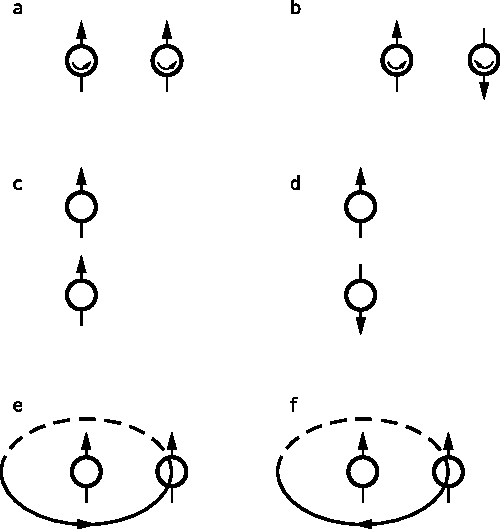
\includegraphics[width=0.6\linewidth]{fyz_fig183.pdf}
      \caption{Síla mezi dvěma protony závisí na všech možných parametrech.
              (\cite[s.~148]{Feynman02}).}
      \label{fyz:fig183}
    \end{figure}

    \begin{figure}[ht!]  %\ref{fyz:fig184}
      \centering
      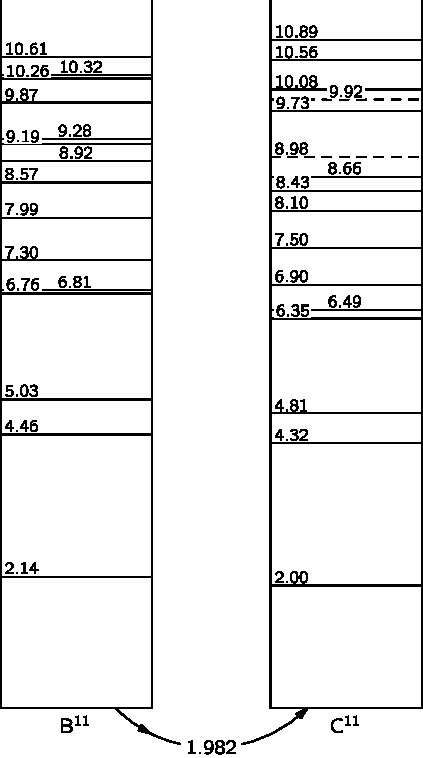
\includegraphics[width=0.6\linewidth]{fyz_fig184.pdf}
      \caption{Energetické hladiny jader \ce{^{11}B} a \ce{^{11}C} (hodnty udané v
              \si{\mega\electronvolt}). Základní stav \ce{^{11}C} leží o
              \SI{1.982}{\mega\electronvolt} výše než základní stav \ce{^{11}B}
              (\cite[s.~149]{Feynman02}).}
      \label{fyz:fig184}
    \end{figure}
    
  \section{Energie v elektrostatickém poli}\label{fyz:IIchapVIsecV}

    \begin{figure}[ht!]  %\ref{fyz:fig185}
      \centering
      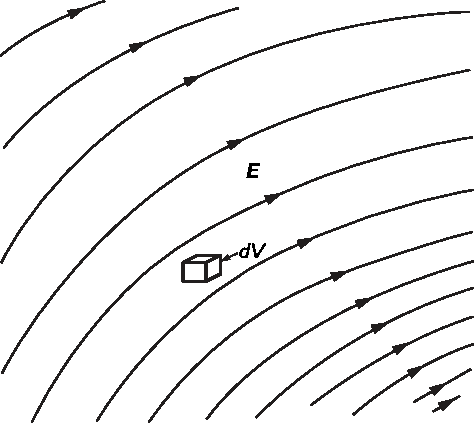
\includegraphics[width=0.6\linewidth]{fyz_fig185.pdf}
      \caption{Každý element objemu \(\dd{V} = \dd{x}\dd{y}\dd{z}\) v elektrickém  poli obsahuje
      energii \(\varepsilon_0/2E^2\dd{V}\) (\cite[s.~154]{Feynman02}).}
      \label{fyz:fig185}
    \end{figure}
    
  \section{Energie bodového náboje}\label{fyz:IIchapVIsecVI}

\todo[inline]{Kapitola fey2ch08 je nedodělaná, obsahuje pouze obrázky}
%} %tikzset
%~~~~~~~~~~~~~~~~~~~~~~~~~~~~~~~~~~~~~~~~~~~~~~~~~~~~~~~~~~~~~~~~~~~~~~~~~~~~~~~~~~~~~~~~~~~~~~~~~~